A major biological application of confocal fluorescence microscopy is the determination of binding fractions between two types of molecules. One method to do so is called \glsfirst{TCCD}. The idea of \gls{TCCD} is that a dye-labeled molecule diffusing through the confocal detection volume causes an intensity peak in the corresponding channel. If there are observed two peaks in both channels at the same time, it can be concluded that there were both fluorescent dyes present in the confocal detection volume. This can be caused by two separate molecules inside the confocal detection volume at the same time, which is called a chance coincidence. However, if the sample concentration is low enough, it is more likely that the coinciding peaks were caused by a chemical complex of the two molecule types. Since the number of non-coincident peaks for both channels is known, \gls{TCCD} allows the calculation of the binding fraction for both molecule types \cite{Orte2010}.\\

Typically, \gls{TCCD} underestimates the binding fraction because the confocal detection volumes for both channels have a different size and do not overlap completely. Usually, the red confocal detection volume is larger than the blue one. This situation is depicted in Figure~\ref{fig:ConfocalVolumeTrajectories}. Three types of trajectories through the confocal detection volumes can be distinguished. If the path of the diffusing molecule only goes through the edge of the red confocal detection volume, it is a borderline trajectory (I). A path through the center of the red confocal detection volume but only through the edge of the blue one is called peripheral trajectory (II). A central trajectory (III) is present if the path goes through the center of both confocal detection volumes. Because of this situation, a complex of both molecule types can pass the confocal detection volume of one channel without causing an intensity peak in the other channel, which leads to an underestimation of the binding fraction. An approach to take the different confocal detection volumes into account is called \glsfirst{BTCCD} \cite{Hoefig2020}.\\ 

\begin{figure}[h]
	\centering
	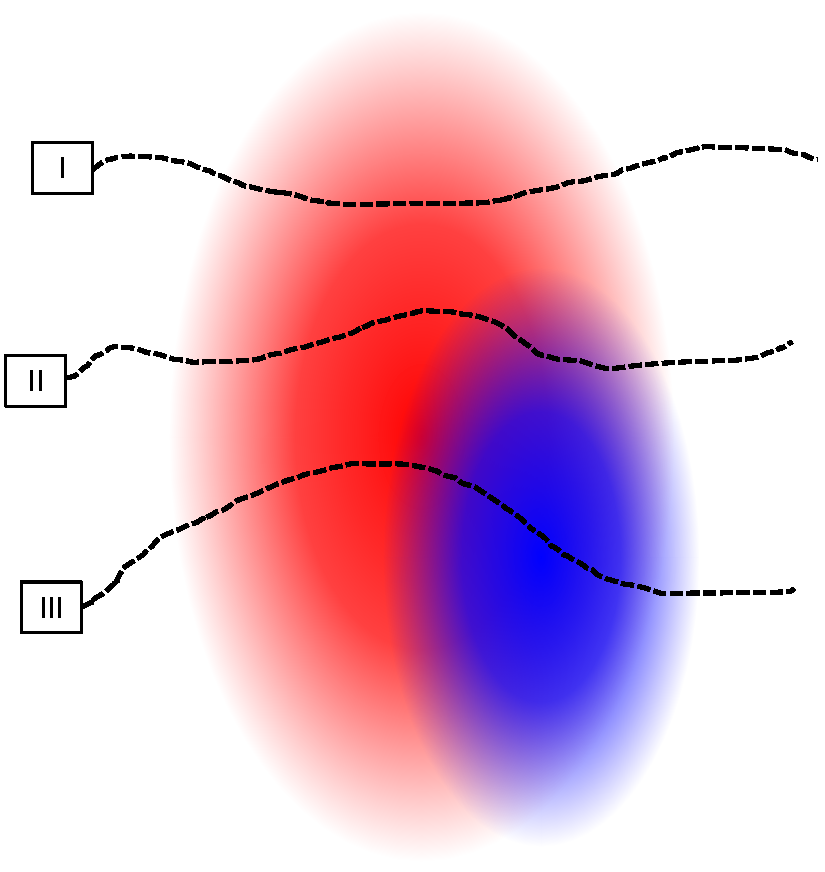
\includegraphics[height= 6.6cm]{ConfocalVolumeTrajectories.pdf}
	\caption[Different size and incomplete overlap of confocal detection volumes]{Red and blue confocal detection volume. Typically, the confocal detection volumes have a different size and do not overlap completely. Therefore, borderline (I), peripheral (II), and central trajectories (III) can be distinguished \cite{Hoefig2020}.}
	\label{fig:ConfocalVolumeTrajectories}
\end{figure}

This section is dedicated to the principles of \gls{BTCCD}. First of all, in Section~\ref{Section:DeterminationOfCoincidenceFraction}, the procedure to determine the coincidence fraction is described in detail. Since chance coincidences become relevant for \gls{BTCCD} even for low concentrations, in Section~\ref{Section:CorrectionForChanceCoincidences} an existing analytic approach to correct for them is presented. Finally, in Section~\ref{Section:DerivedQuantities}, mathematical expressions for three important quantities that occur during the application of \gls{BTCCD} are derived.

\subsection{Determination of Coincidence Fraction} \label{Section:DeterminationOfCoincidenceFraction}

The procedure to determine the coincidence fraction with \gls{BTCCD} taking the different trajectory types into account consists of four steps:

\subsubsection*{1 Calculate \gls{IPL} Time Trace}

By using the \glsfirst{IPL} time trace instead of the intensity trace, \gls{BTCCD} takes advantage of the single-photon detection of the \glspl{AVD}. The \gls{IPL} time trace can be calculated from the macro time $t(n)$, where $n$ indicates the number of the detected photon. It is defined by
\begin{equation}
	IPL(n) = t(n) - t(n-1),
\end{equation}
such that for every detected photon (except the first one) the time difference to the occurrence of the previous photon is calculated. To stabilize the \gls{IPL} time trace, a moving average 
\begin{equation}
	IPL_m(n) = \sum_{i = n-m}^{n+m} \frac{IPL(i)}{2m + 1}
\end{equation}
is applied. Throughout this thesis, $m$ was set to $2$. It has been shown that the results of \gls{BTCCD} do not depend significantly on the choice of $m$ \cite{Hoefig2020}. An excerpt of an \gls{IPL} time trace can be found in Figure~\ref{fig:IPLTrace}. There, the raw \gls{IPL} time trace as well as the smoothed one is shown.

\subsubsection*{2 Set Burst Threshold}

For the determination of the coincidence fraction, it is necessary to define what is considered as a photon burst, corresponding to a peak in the intensity trace. For this purpose, burst thresholds $IPL^{tre}$ for both channels are defined. Every time the \gls{IPL} time trace falls below this threshold, a photon burst is present. As illustrated in Figure~\ref{fig:ConfocalVolumeTrajectories} above, three types of trajectories through the confocal detection volume can be distinguished. They are also identifiable in the \gls{IPL} time trace as shown in Figure~\ref{fig:IPLTrace}. A borderline trajectory (I) leads to a dim burst in the red channel, while there is no burst in the blue one. If the blue \gls{IPL} time trace drops slightly below the burst threshold, the molecule complex followed a peripheral trajectory (II). A central trajectory (III) corresponds to bright bursts in both channels. 

Substantial quantities that follow from the definition of a photon burst are the molecular brightness $MB$ and the dwell time $\tau_d$. The dwell time is the width of a burst, while the molecular brightness is given by
\begin{equation}
	MB = \frac{N_{\gamma}}{\tau_d},
\end{equation}
where $N_{\gamma}$ is the number of photons in the burst with dwell time $\tau_d$. Both quantities can be calculated for every single burst. In practice, their average values for all bursts in one channel are of interest. Therefore, in the following, $\left\langle MB \right\rangle$ and $\left\langle \tau_d \right\rangle$ denote these average values, and it is not always explicitly stated that they are calculated from a certain number of bursts. For the analysis of the measurements, the brightness thresholds were set such that $\left\langle MB \right\rangle$ and $\left\langle \tau_d \right\rangle$ are in rough agreement with the values obtained by \gls{FCS}.~\footnote{Although \gls{FCS} uses the intensity time trace, an average dwell time can be derived from the measured diffusion coefficient: $\left\langle \tau_d \right\rangle = r_0^2/ (4D)$. Then, the molecular brightness $\left\langle MB \right\rangle$ is simply the average number of photons in an intensity peak $\left\langle N_{\gamma} \right\rangle$ divided by the average dwell time $\left\langle \tau_d \right\rangle$ as well as by the average number of molecules inside the confocal detection volume $\left\langle N \right\rangle$: $\left\langle MB \right\rangle = \left\langle N_{\gamma} \right\rangle/ (\left\langle \tau_d \right\rangle \left\langle N \right\rangle)$. For \gls{FCS}, the single quantities are averaged before calculating the molecular brightness , whereas \gls{BTCCD} allows the calculation of the molecular brightness for every burst \cite{Schwille2001}.}
 
\begin{figure}[h]
	\centering
	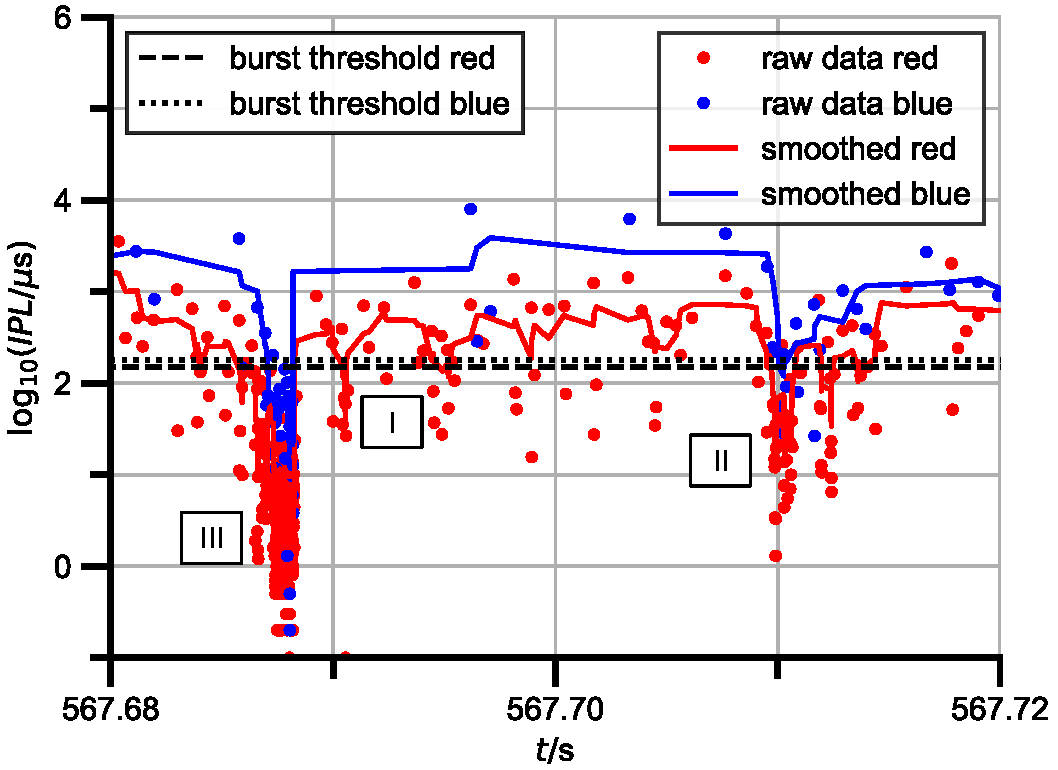
\includegraphics[width=4in]{IPLTrace.pdf}
	\caption[\gls{IPL} time trace and definition of bursts]{\gls{IPL} time trace calculated from macro time trace. Photon bursts are distinguished from the background by a burst threshold. Bursts resulting from borderline (I), peripheral (II), and central trajectories (III) can be identified, corresponding to Figure~\ref{fig:ConfocalVolumeTrajectories}. The data is taken from a measurement of dual-labeled \gls{dsDNA}, see Section~\ref{Section:BTCCD_Measurement_Dependencies}.}
	\label{fig:IPLTrace}
\end{figure}

Every measurement with the confocal microscope is, to a certain degree, disturbed by external sources, e.g., dark currents in the detection electronics. If the effect is not too large, the associated \gls{IPL} values are larger than those caused by a molecule passing through the confocal detection volume. The average background $\left\langle IPL^{bg} \right\rangle$ can be estimated by plotting a histogram of the measured \gls{IPL} values. An example of the red channel can be found in Figure~\ref{fig:IPLBackground_Red}. The histogram reveals two separate populations. The right population corresponds to higher \gls{IPL} values and reflects thus the background. Since the right population is almost symmetrical, its maximum can be taken as a value for $\left\langle IPL^{bg} \right\rangle$. The corresponding background characterization for the blue channel is illustrated in Figure~\ref{fig:IPLBackground_Blue}. The burst threshold $IPL^{tre}$ should be smaller than the average background to prevent the misidentification of the background as bursts.
\clearpage

\begin{figure}[h]
	\centering
	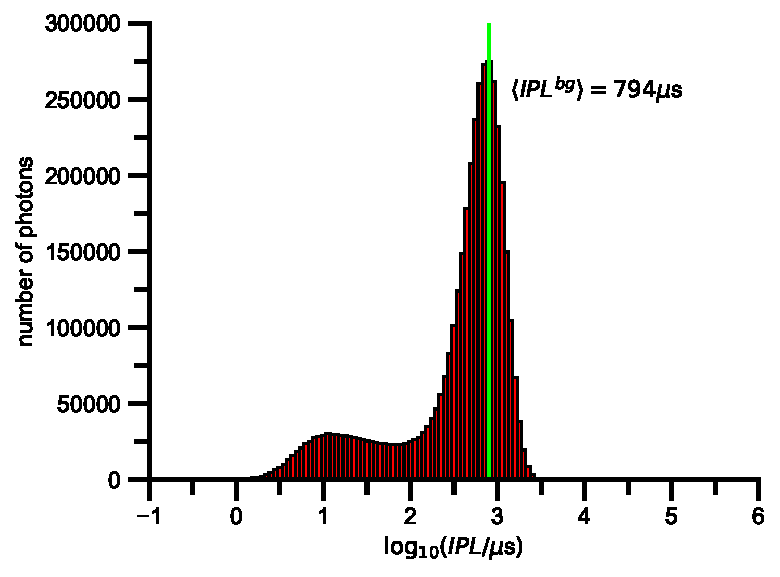
\includegraphics[width=4in]{dlDNA_IPD_Red.pdf}
	\caption[Determination of background in \gls{IPL} time trace for red channel]{Histogram of \gls{IPL} values for the red channel. The right population reflects the background. In this case, it is characterized by $\left\langle IPL^{bg} \right\rangle = \SI{794}{\micro\second}$ as indicated by the vertical green line. The data is taken from a measurement of dual-labeled \gls{dsDNA}, see Section~\ref{Section:BTCCD_Measurement_Dependencies}.}
	\label{fig:IPLBackground_Red}
\end{figure}                       

\subsubsection*{3 Apply Different Brightness Thresholds}

Every burst defined by the burst threshold in the \gls{IPL} time trace consists of a certain number of photons. Dim bursts of type I and II contain only a small number of photons. The scope of \gls{BTCCD} is to exclude these bursts in order to prevent an underestimation of the coincidence fraction. To do so, the bursts are further selected by choosing only bursts with more than a minimum number of photons $N_{\gamma,min}$, called brightness threshold. To ensure the comparability between both channels, the brightness threshold is usually normalized on the average number of photons $\left\langle N_{\gamma,0} \right\rangle$ in the initial bursts for each channel. In the following, the normalized brightness threshold is called $n_{br}$ and is given by
\begin{equation}
	n_{br} = \frac{N_{\gamma,min}}{\left\langle N_{\gamma,0} \right\rangle}.
\end{equation}\\

To calculate the coincidence fraction for the bursts selected by $n_{br}$ in the red channel, the total number of selected red bursts $B_{R}$, as well as the number of coincident bursts $B_{RB}$ has to be counted. A burst in the red channel is coincident if its start or end time falls between the start and end time of a blue burst. Here, all initial blue bursts are considered since the brightness threshold for both channels is applied separately. Then, the coincidence fraction for the red channel is given by
\begin{equation}
	f_{RB}(n_{br}) = \frac{B_{RB}(n_{br})}{B_{R}(n_{br})}.
\end{equation}
For the blue channel, an analogous consideration yields
\begin{equation}
f_{BR}(n_{br}) = \frac{B_{BR}(n_{br})}{B_{B}(n_{br})}.
\end{equation}
Since a count of bursts is a Poisson distributed number, the uncertainty on these quantities are given by
\begin{equation} \label{Equation:UncertaintyCoincidenceFractionRed}
	\sigma_{f_{RB}}(n_{br}) = f_{RB}(n_{br}) \cdot \sqrt{\frac{1}{B_{RB}(n_{br})} + \frac{1}{B_{R}(n_{br})}}
\end{equation}
and
\begin{equation}
	\sigma_{f_{BR}}(n_{br}) = f_{BR}(n_{br}) \cdot \sqrt{\frac{1}{B_{BR}(n_{br})} + \frac{1}{B_{B}(n_{br})}}.
\end{equation}
An example for the calculation of the coincidence fraction as a function of $n_{br}$ is illustrated in Figure~\ref{fig:CoincidenceFraction_dlDNA}. There, the exclusion of borderline (I) and peripheral trajectories (II) can be observed by the increase of the coincidence fractions for lower brightness thresholds. For higher brightness thresholds, the curves saturate since only central trajectories (III) remain.

\begin{figure}[h]
	\centering
	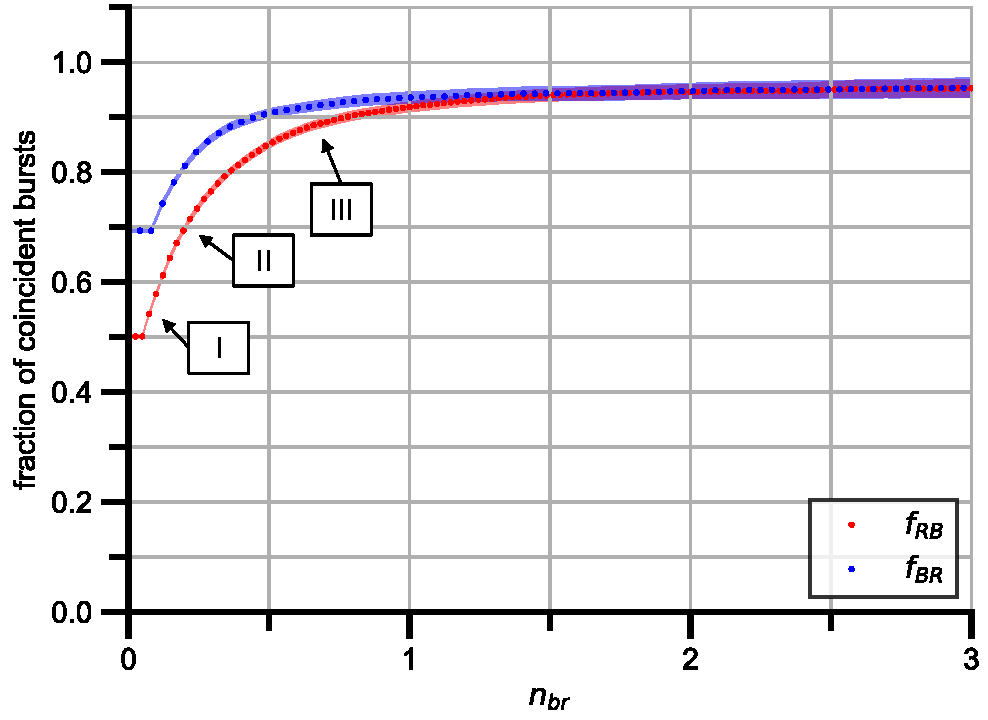
\includegraphics[width=4in]{ConcidenceFraction_dlDNA.pdf}
	\caption[Coincidence fraction as a function of $n_{br}$]{Fraction of coincident bursts for both channels as a function of $n_{br}$. For large values of $n_{br}$, the curves saturate since borderline (I) and peripheral trajectories (II) have been excluded, compare to Figures~\ref{fig:ConfocalVolumeTrajectories} and \ref{fig:IPLTrace}. The data is taken from a measurement of dual-labeled \gls{dsDNA}, see Section~\ref{Section:OptimalNumberOfBursts_Measurement}.}
	\label{fig:CoincidenceFraction_dlDNA}
\end{figure}

The application of \gls{BTCCD} effectively decreases the confocal detection volume. For a given brightness threshold, the average number of molecules inside the confocal detection volume of one channel can be calculated from the number of selected bursts $B$, the total measurement time $T$, and the dwell time $\left\langle \tau_d \right\rangle$ according to \cite{Hoefig2020}
\begin{equation} \label{Equation:AverageNumberOfMolecules}
	\left\langle N \right\rangle (n_{br})  = -ln\left(1 - \frac{B(n_{br}) \cdot \left\langle \tau_d \right\rangle(n_{br})}{T}\right).
\end{equation}
In Section~\ref{Appendix:UncertaintyDwellTime}, the uncertainties on the relevant quantities $\left\langle \tau_d \right\rangle$, $\left\langle N \right\rangle$, and $\left\langle MB \right\rangle$ are derived.

\subsubsection*{4 Find Optimal Brightness Threshold}

Having determined the coincidence fraction for different burst thresholds, the question remains which coincidence fraction should be taken as the ideal one. For larger $n_{br}$, the uncertainty on the coincidence fraction increases significantly since the number of bursts decreases. However, for lower $n_{br}$ not all trajectories of type I and II have been excluded. Therefore, a compromise between precision and accuracy has to be found. For the red channel, the precision is defined as the relative uncertainty:
\begin{equation} \label{Equation:PrecisionCoincidenceFractionRed}
	\frac{\sigma_{f_{RB}}(n_{br})}{f_{RB}(n_{br})} = \sqrt{\frac{1}{B_{RB}(n_{br})} + \frac{1}{B_{R}(n_{br})}}.
\end{equation} 
The accuracy is the deviation of the coincidence fraction at a certain $n_{br}$ from its value $f_{RB,high}$ at the highest brightness threshold. It is given by
\begin{equation}
	\frac{\Delta f_{RB}(n_{br})}{f_{RB}(n_{br})} = \frac{f_{RB,high} - f_{RB}(n_{br})}{f_{RB}(n_{br})}.
\end{equation}
For the blue channel, similar expressions are obtained. To find the optimal brightness threshold $n_{br, opt}$, the intersection between precision and accuracy has to be determined. An example for the red channel can be found in Figure~\ref{fig:OptimalBrightnessThresholdRedChannel_dlDNA}. The search for the optimal brightness threshold for the blue channel is illustrated in Figure~\ref{fig:OptimalBrightnessThresholdBlueChannel_dlDNA}.

\begin{figure}[h]
	\centering
	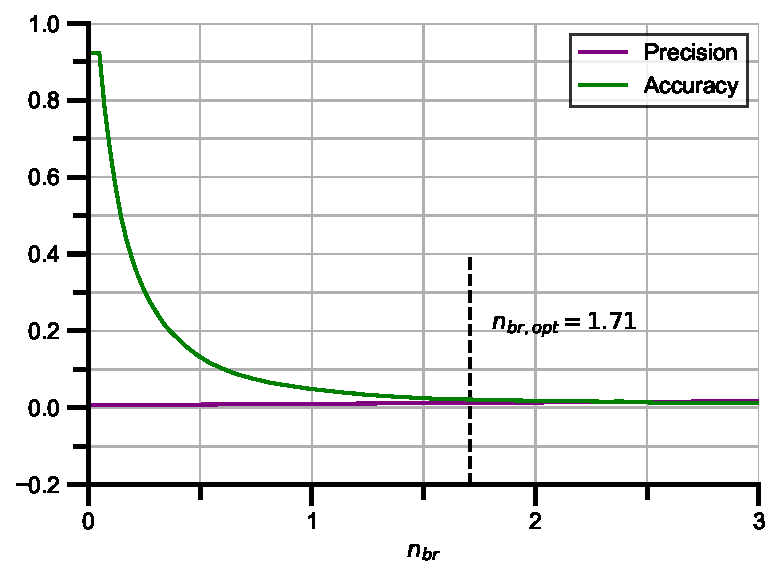
\includegraphics[width=4in]{OptimalBrightnessThresholdRedChannel_dlDNA.pdf}
	\caption[Search for optimal brightness threshold $n_{br, opt}$ for red channel]{Search for the optimal brightness threshold $n_{br, opt}$ for the red channel. $n_{br, opt}$ is given by the intersection of precision and accuracy. The data is taken from a measurement of dual-labeled \gls{dsDNA}, see Section~\ref{Section:OptimalNumberOfBursts_Measurement}. In this case, $n_{br, opt}=\num{1.71}$ leads to a coincidence fraction of $f_{RB}(n_{br, opt}) = \SI{94.3 +- 1.2}{\percent}$.}
	\label{fig:OptimalBrightnessThresholdRedChannel_dlDNA}
\end{figure}

\subsection{Correction for Chance Coincidences} \label{Section:CorrectionForChanceCoincidences}

A coincidence will be counted by the procedure presented so far if two or more molecules with a different dye-labeling are simultaneously inside the confocal detection volume. This leads to an overestimation of the binding fraction since the coincidence may not be caused by an actual binding between different molecule types. The probability of the occurrence of such chance coincidences depends on the sample concentration. If the average number of molecules inside the confocal detection volume for each channel is lower than \num{0.03}, the probability for more than one molecule present in the confocal detection volume is smaller than \SI{0.1}{\percent} \cite{Hoefig2020}. Therefore, chance coincidences do not need to be considered for \gls{TCCD}. However, by applying \gls{BTCCD}, dim bursts are excluded. For the remaining subset of bright bursts, the molecules stay for a relatively long time in the confocal detection volume. Thus, the probability that another molecule enters the confocal detection volume increases. Hence, for \gls{BTCCD}, even for low sample concentrations, the effect of chance coincidences cannot be neglected.\\

In \cite{Hoefig2020}, an approach to correct for chance coincidences has been proposed. To estimate the chance coincidence fraction, the average dwell time $\left\langle \tau_d \right\rangle$ as well as the average number of molecules inside the confocal detection volume $\left\langle N \right\rangle$ have to be known for both channels. $\left\langle \tau_d \right\rangle$ is directly accessible, while $\left\langle N \right\rangle$ is given by Equation~\ref{Equation:AverageNumberOfMolecules}.
If the probability for more than two molecules of different colors inside the confocal detection volume is neglected, the corrected coincidence fraction for the red channel can be expressed as
\begin{equation} \label{Equation:CorrectedCoincidenceFractionRed}
f_{RB}^{cor}(n_{br}) = \frac{f_{RB}(n_{br}) - f_{RB, 0}^{chance}(n_{br})}{1 - f_{RB, 0}^{chance}(n_{br})},
\end{equation}
where
\begin{equation} \label{Equation:ChanceCoincidenceFractionRed}
f_{RB, 0}^{chance}(n_{br}) = 1 - \exp\left\{-\left\langle N_B \right\rangle (0) \cdot \left(\frac{\left\langle \tau_d^R\right\rangle (n_{br})}{\left\langle \tau_d^B \right\rangle (0)} + 1\right)\right\}.
\end{equation}
Both $\left\langle N_B \right\rangle$ and $\left\langle \tau_d^B \right\rangle$ do not depend on the brightness threshold since the procedure of \gls{BTCCD} is applied separately for both channels. The corrected coincidence fraction for the blue channel is analogously given by
\begin{equation}
f_{BR}^{cor}(n_{br}) = \frac{f_{BR}(n_{br}) - f_{BR, 0}^{chance}(n_{br})}{1 - f_{BR, 0}^{chance}(n_{br})},
\end{equation}
where
\begin{equation}
f_{BR, 0}^{chance}(n_{br}) = 1 - \exp\left\{-\left\langle N_R \right\rangle (0) \cdot \left(\frac{\left\langle \tau_d^B \right\rangle (n_{br})}{\left\langle \tau_d^R \right\rangle (0)} + 1\right)\right\}.
\end{equation}
A detailed derivation of the uncertainties on $f_{RB}^{cor}$ and $f_{BR}^{cor}$ can be found in Section~\ref{Appendix:UncertaintyOnChanceCoincidenceCorrection}.

\clearpage

\subsection{Dependencies on Brightness Threshold} \label{Section:DerivedQuantities}

In this section, the dependencies of $\left\langle \tau_d \right\rangle$, $\left\langle N \right\rangle$, and $\left\langle MB \right\rangle$ on the brightness threshold $n_{br}$ are derived. The obtained theoretical results are compared with experimental data in Chapter~\ref{Chapter:DependenciesOnBrightnessThreshold}.

\subsubsection{Dwell Time}\label{Section:DwellTime}

A certain number of photons is emitted if a molecule passes through the confocal detection volume. On average, this number is proportional to the minimum number of photons $N_{\gamma,min}$ defined by the burst threshold. Since the emission of photons by a fluorophore is a statistical process, an average time $\Delta t_{\gamma}'$ between the emission of two photons can be defined. Let $\tau_d^0$ be the average duration of a burst for $N_{\gamma,min}=0$. Then, the average dwell time as a function of $N_{\gamma,min}$ can be expressed by
\begin{equation}
	\left\langle \tau_d \right\rangle (N_{\gamma,min}) = \Delta t_{\gamma}'(N_{\gamma,min}) \cdot n_{br} + \tau_d^0
\end{equation}
since, on average, every photon increases the dwell time by $\Delta t_{\gamma}'$. In general, $\Delta t_{\gamma}'$ depends on $N_{\gamma,min}$ since, for dim bursts, the time between the emission of two photons is larger than for bright bursts. However, for larger $N_{\gamma,min}$, most dim bursts are excluded, and only bright bursts remain. Since bright bursts correspond to central trajectories through the confocal detection volume, a further increase of $N_{\gamma,min}$ does not change the time between the emission of two photons significantly. \\ 

The normalized brightness threshold is given by $n_{br} = N_{\gamma,min}/ \left\langle N_{\gamma,0} \right\rangle$, where $\left\langle N_{\gamma,0} \right\rangle$ is the average number of photons in the initial bursts. Hence, the dependency of the average dwell time on $n_{br}$ is described by
\begin{equation}
	\left\langle \tau_d \right\rangle (n_{br}) = \Delta t_{\gamma}(n_{br}) \cdot n_{br} + \tau_d^0,
\end{equation}
where $\Delta t_{\gamma}(n_{br}) = \Delta t_{\gamma}'(N_{\gamma,min}) \cdot \left\langle N_{\gamma,0} \right\rangle$. All in all, it is expected that, for large enough $n_{br}$, $\Delta t_{\gamma}$ is constant, and a linear function with constant slope describes the dwell time.

\subsubsection{Number of Molecules}
An increase of $n_{br}$ effectively decreases the confocal detection volume, and leads, thus, also to a decrease of $\left\langle N \right\rangle$. To examine the specific form of decrease, suppose that a certain increase of $n_{br}$ decreases the confocal detection volume by $\Delta V$. If $\left\langle N \right\rangle$ is large, many molecules are in the volume element $\Delta V$. In contrast, for a small $\left\langle N \right\rangle$, only a few molecules are in the exact same volume element. The number of molecules that is excluded by decreasing the confocal detection volume depends, thus, on $\left\langle N \right\rangle$ itself. This situation can be described by the differential equation
\begin{equation}
	\diff{\left\langle N \right\rangle}{n_{br}}(n_{br}) = -\frac{1}{n} \left\langle N \right\rangle (n_{br}),
\end{equation}
where $1/ n$ is a proportionality constant. Its solution is given by 
\begin{equation}
	\left\langle N \right\rangle (n_{br}) = N^0 e^{-n_{br}/ n},
\end{equation}
where $N^0$ is the average number of molecules for $n_{br} = 0$.

\subsubsection{Molecular Brightness}

The molecular brightness is a relative quantity since it describes the number of photons in a burst in relation to the dwell time. For large $n_{br}$, the number of photons in a burst, and the dwell time is proportional to $n_{br}$, see above. Therefore, the molecular brightness saturates at some value $MB^{max}$. The molecular brightness $MB^0$ for $n_{br} = 0$ is smaller than $MB^{max}$ since dim bursts decrease the molecular brightness. Furthermore, $\left\langle MB \right\rangle$ should be a smooth function that connects $MB^0$ with $MB^{max}$ since there is no particular $n_{br}$ for which suddenly all dim bursts are excluded. This means that the slope of $\left\langle MB \right\rangle$ depends on the difference between $MB^{max}$ and the current value of $\left\langle MB \right\rangle$ because the derivative of $\left\langle MB \right\rangle$ has to approach $0$. Thus, $\left\langle MB \right\rangle$ is described by the non-homogeneous differential equation
\begin{equation}
	\diff{\left\langle MB \right\rangle}{n_{br}}(n_{br}) = \frac{1}{n} \cdot \left(MB^{max} - \left\langle MB \right\rangle(n_{br})\right),
\end{equation}
where $1/ n$ is a proportionality constant. Its solution is given by 
\begin{equation}
	\left\langle MB \right\rangle(n_{br}) = MB^0 + \Delta MB (1 - e^{-n_{br}/ n}),
\end{equation}
where $MB^{max} - MB^0$.
